% Autor: Leonhard Segger, Alexander Neuwirth
% Datum: 2017-10-30
\documentclass[
	% Papierformat
	a4paper,
	% Schriftgröße (beliebige Größen mit „fontsize=Xpt“)
	12pt,
	% Schreibt die Papiergröße korrekt ins Ausgabedokument
	pagesize,
	% Sprache für z.B. Babel
	ngerman
]{scrartcl}

% Achtung: Die Reihenfolge der Pakete kann (leider) wichtig sein!
% Insbesondere sollten (so wie hier) babel, fontenc und inputenc (in dieser
% Reihenfolge) als Erstes und hyperref und cleveref (Reihenfolge auch hier
% beachten) als Letztes geladen werden!

% Silbentrennung etc.; Sprache wird durch Option bei \documentclass festgelegt
\usepackage{babel}
% Verwendung der Zeichentabelle T1 (Sonderzeichen etc.)
\usepackage[T1]{fontenc}
% Legt die Zeichenkodierung der Eingabedatei fest, z.B. UTF-8
\usepackage[utf8]{inputenc}
% Schriftart
\usepackage{lmodern}
% Zusätzliche Sonderzeichen
\usepackage{textcomp}

% Mathepaket (intlimits: Grenzen über/unter Integralzeichen)
\usepackage[intlimits]{amsmath}
% Ermöglicht die Nutzung von \SI{Zahl}{Einheit} u.a.
\usepackage{siunitx}
% Zum flexiblen Einbinden von Grafiken (\includegraphics)
\usepackage{graphicx}
% Abbildungen im Fließtext
\usepackage{wrapfig}
% Abbildungen nebeneinander (subfigure, subtable)
\usepackage{subcaption}
% Funktionen für Anführungszeichen
\usepackage{csquotes}
% Zitieren, Bibliographie
\usepackage{biblatex}

% Verlinkt Textstellen im PDF-Dokument
\usepackage[unicode]{hyperref}
% "Schlaue" Referenzen (nach hyperref laden!)
\usepackage{cleveref}
% Zur Darstellung von Webadressen
\usepackage{url}
%chemische Formeln
\usepackage[version=4]{mhchem}
% siunitx: Deutsche Ausgabe, Messfehler getrennt mit ± ausgeben
\usepackage{floatrow}
\floatsetup[table]{capposition=top}
\sisetup{
	locale=DE,
	separate-uncertainty
}
%\bibliography{6Mi_S2_25-10-2017_References}

\begin{document}
	
	\begin{titlepage}
		\centering
		{\scshape\LARGE Versuchsbericht zu \par}
		\vspace{1cm}
		{\scshape\huge M2 - Gekoppelte Pendel\par}
		\vspace{2.5cm}
		{\LARGE Gruppe 6Mi \par}
		\vspace{0.5cm}
		
		{\large Alexander Neuwirth (E-Mail: a\_neuw01@wwu.de) \par}
		{\large Leonhard Segger (E-Mail: l\_segg03@uni-muenster.de) \par}
		\vfill
		
		durchgeführt am 22.11.2017\par
		betreut von\par
		{\large Martin Körsgen}
		
		\vfill
		
		{\large \today\par}
	\end{titlepage}
	\tableofcontents
	\newpage
	
	\section{Kurzfassung}
	Kurzfassung...
	Gekoppelte Pendel
	Doppel Pendel

	\section{Methoden}
	Der Versuch besteht aus zwei Pendeln die mittels verschieden starken Federn gekoppelt werden. Damit beide Pendeln mit der gleiche Eigenfrequenz schwingen, haben wir die Länge der Pendel so angepasst, dass sie auch nach ca. 20 Perioden ohne Kopplung synchron schwingen. Der Kopplungsgrad und die relative Frequenzspaltung wurde statisch sowie dynamisch bestimmt. Bei der statischen Messung wird ein Pendel ausgelenkt und die resultierende Auslenkung des anderen Pendels aufgenommen. Dynamsich ergibt sich der Kopplungsgrad aus den Schwingdauern der Grundschwingungen einer gleichsinnigen und gegensinnigen Bewegung.
	Zum Bestimmen der Schwingdauern wurde ein Ultraschall-Entfernungssensor verwendet, jedoch traten beim Testen der Messapperatur bei Sensorfrequenzen über \SI{50}{Hz} Softwareprobleme auf.

	\noindent{}Das Verhalten eines Doppelpendels wurde beobachtet mit verschiedenen initialen Auslenkungen und Geschwindigkeiten. 
	

	\section{Ergebnisse und Diskussion}
	Analyse der Schwingzeiten über jeweils 60sec, außer bei Schwebungsbestimmung mit 120sec. Graphen?!? \\
	mehr! \\%TODO


	\subsection{Pendel}
	In \cref{SchwingungOhneKopplung} sind in schwarz einzelne Entfernungsmessugnen des Ultraschallsensors sowie ein nicht linearer Fit in rot aufgetragen. 
	Die Schwingdauer $T_0$ eines einzelnen Pendels lässt sich hieraus mit \SI{2,477}{s} bestimmen.

	\begin{figure}[H]
		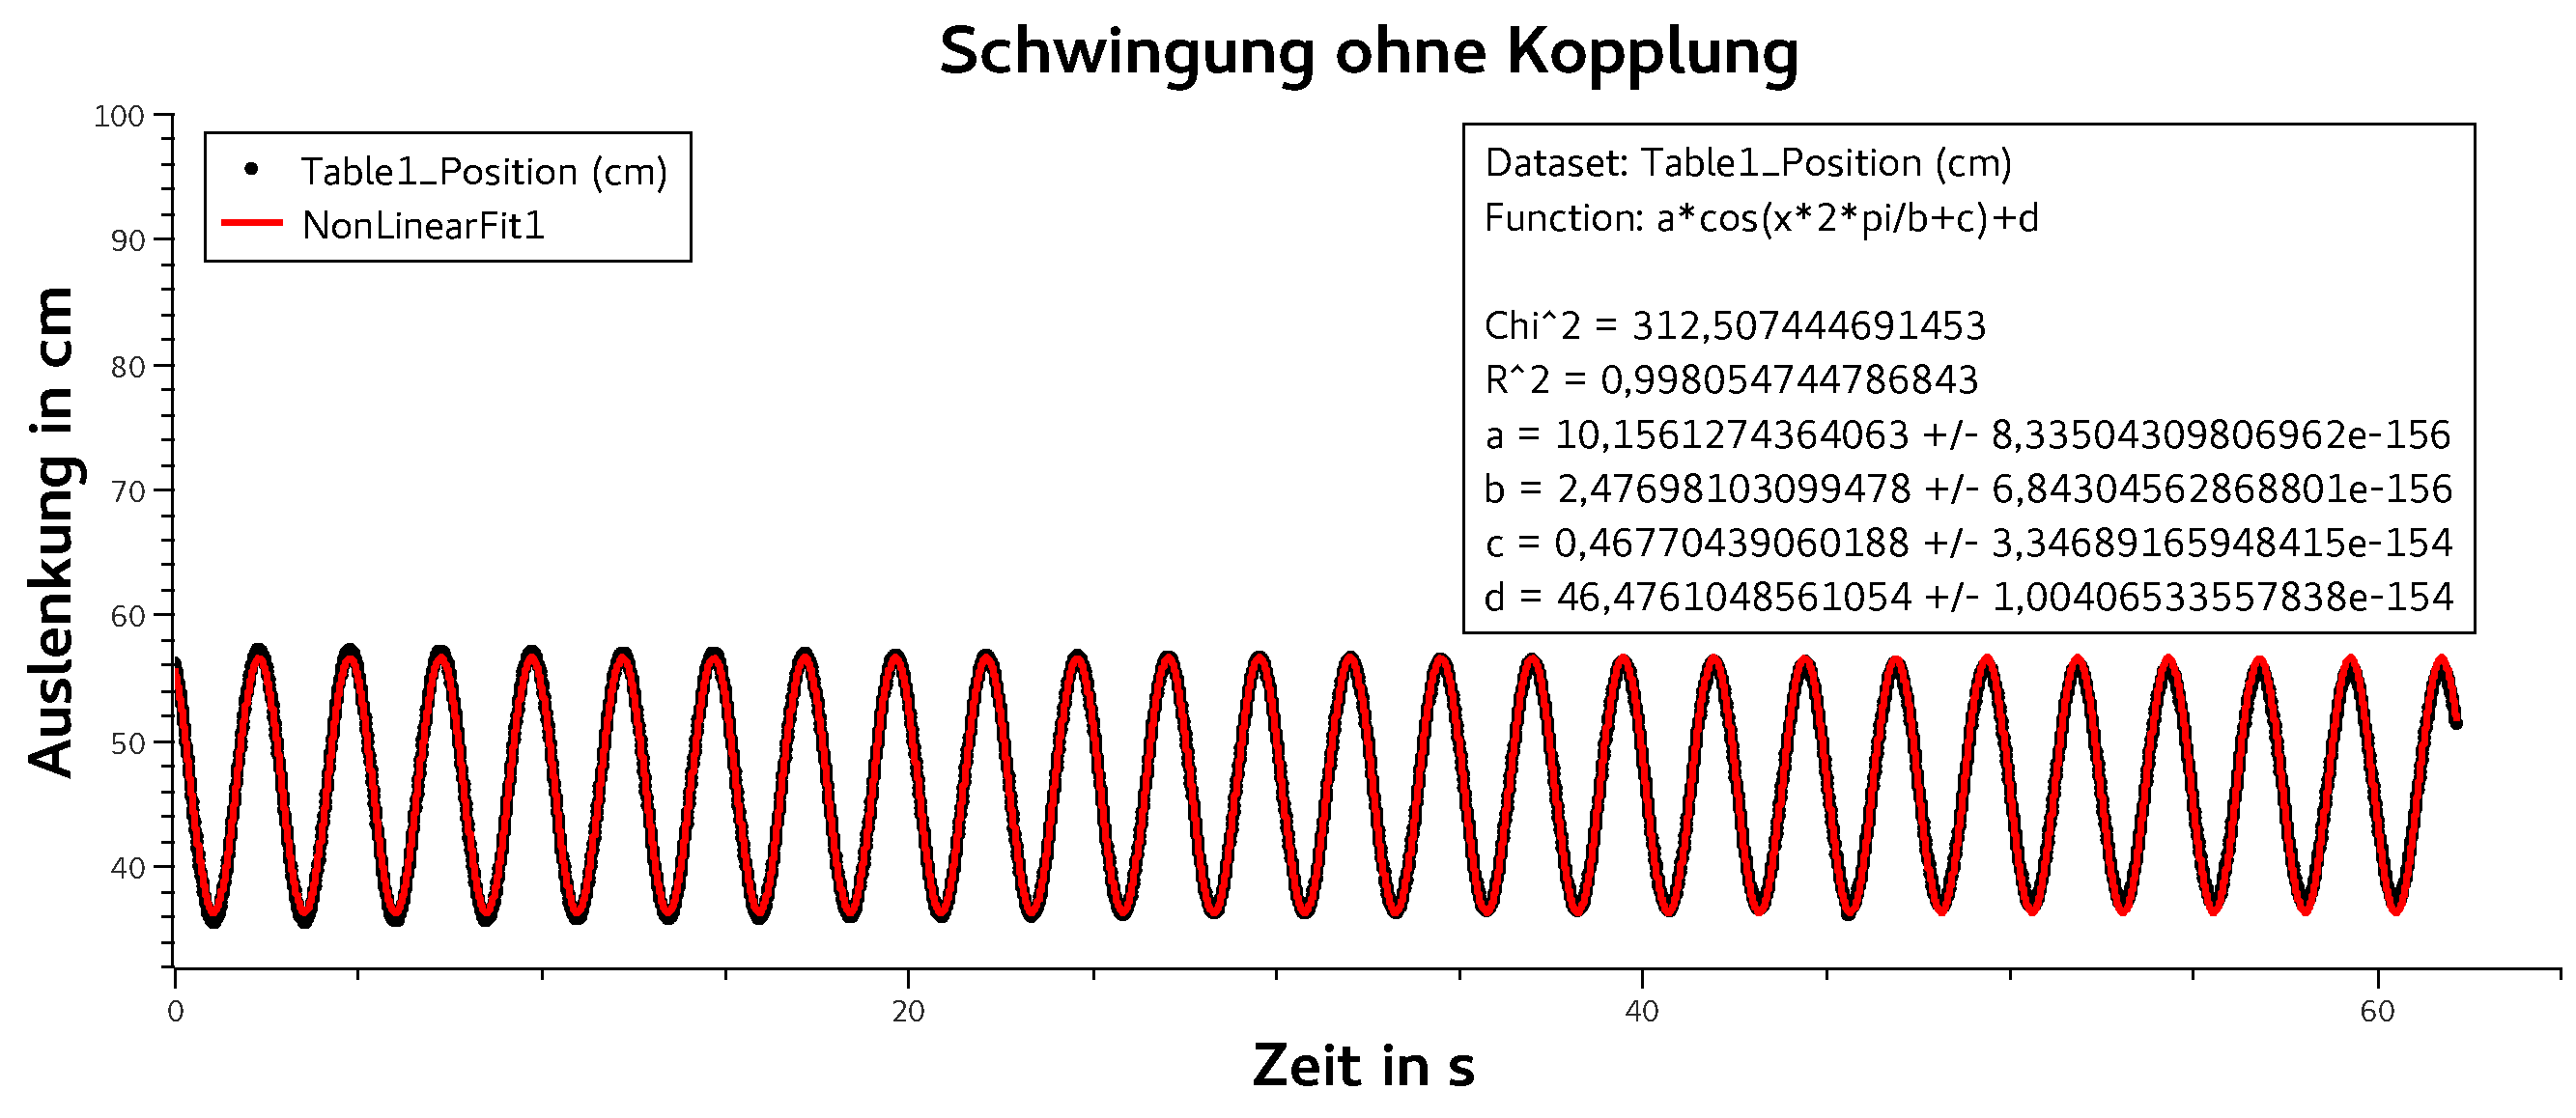
\includegraphics[width=1\textwidth]{SchwingungOhneKopplung}
		\centering
		\caption{Schwingung eines Fadenpendels.}
		\label{SchwingungOhneKopplung}
		\centering
	\end{figure}

	\subsection{Gekoppelte Pendel}
	Bestimmen der Schwingdauern. \\
	Resultierends K. $T_s$ und Frequenzspaltungen \\
	\subsubsection{Statische Bestimmung des Kopplungsgrades}
	Die gegeben Formel für den Kopplungsgrad lautet:
	\begin{equation}
		k = \frac{x_1}{x_2}.
	\end{equation}

	\begin{table}[h]
		\centering
	\begin{tabular}{ r | c | c | c |}
		& Kupfer & Edelstahl  \\ \hline
		$x_1 $ &$\SI{9,8}{cm}$&$\SI{10}{cm}$\\  
		$x_2 $ &$\SI{1,9}{cm}$&$\SI{3,1}{cm}$\\  \hline\hline
		$k$  & $\SI{5,158}{}$ &  $\SI{3,226}{}$ \\ \hline


	\end{tabular}
	\caption{Messwerte beim Auslenken eines Pendels um $x_1$ und der resultierende Ausschlag des gekoppelten Pendels um $x_2$}
	\end{table}

	\subsubsection{Gleichschwingung}

	\subsubsection*{Kupfer}
	\begin{figure}[H]
		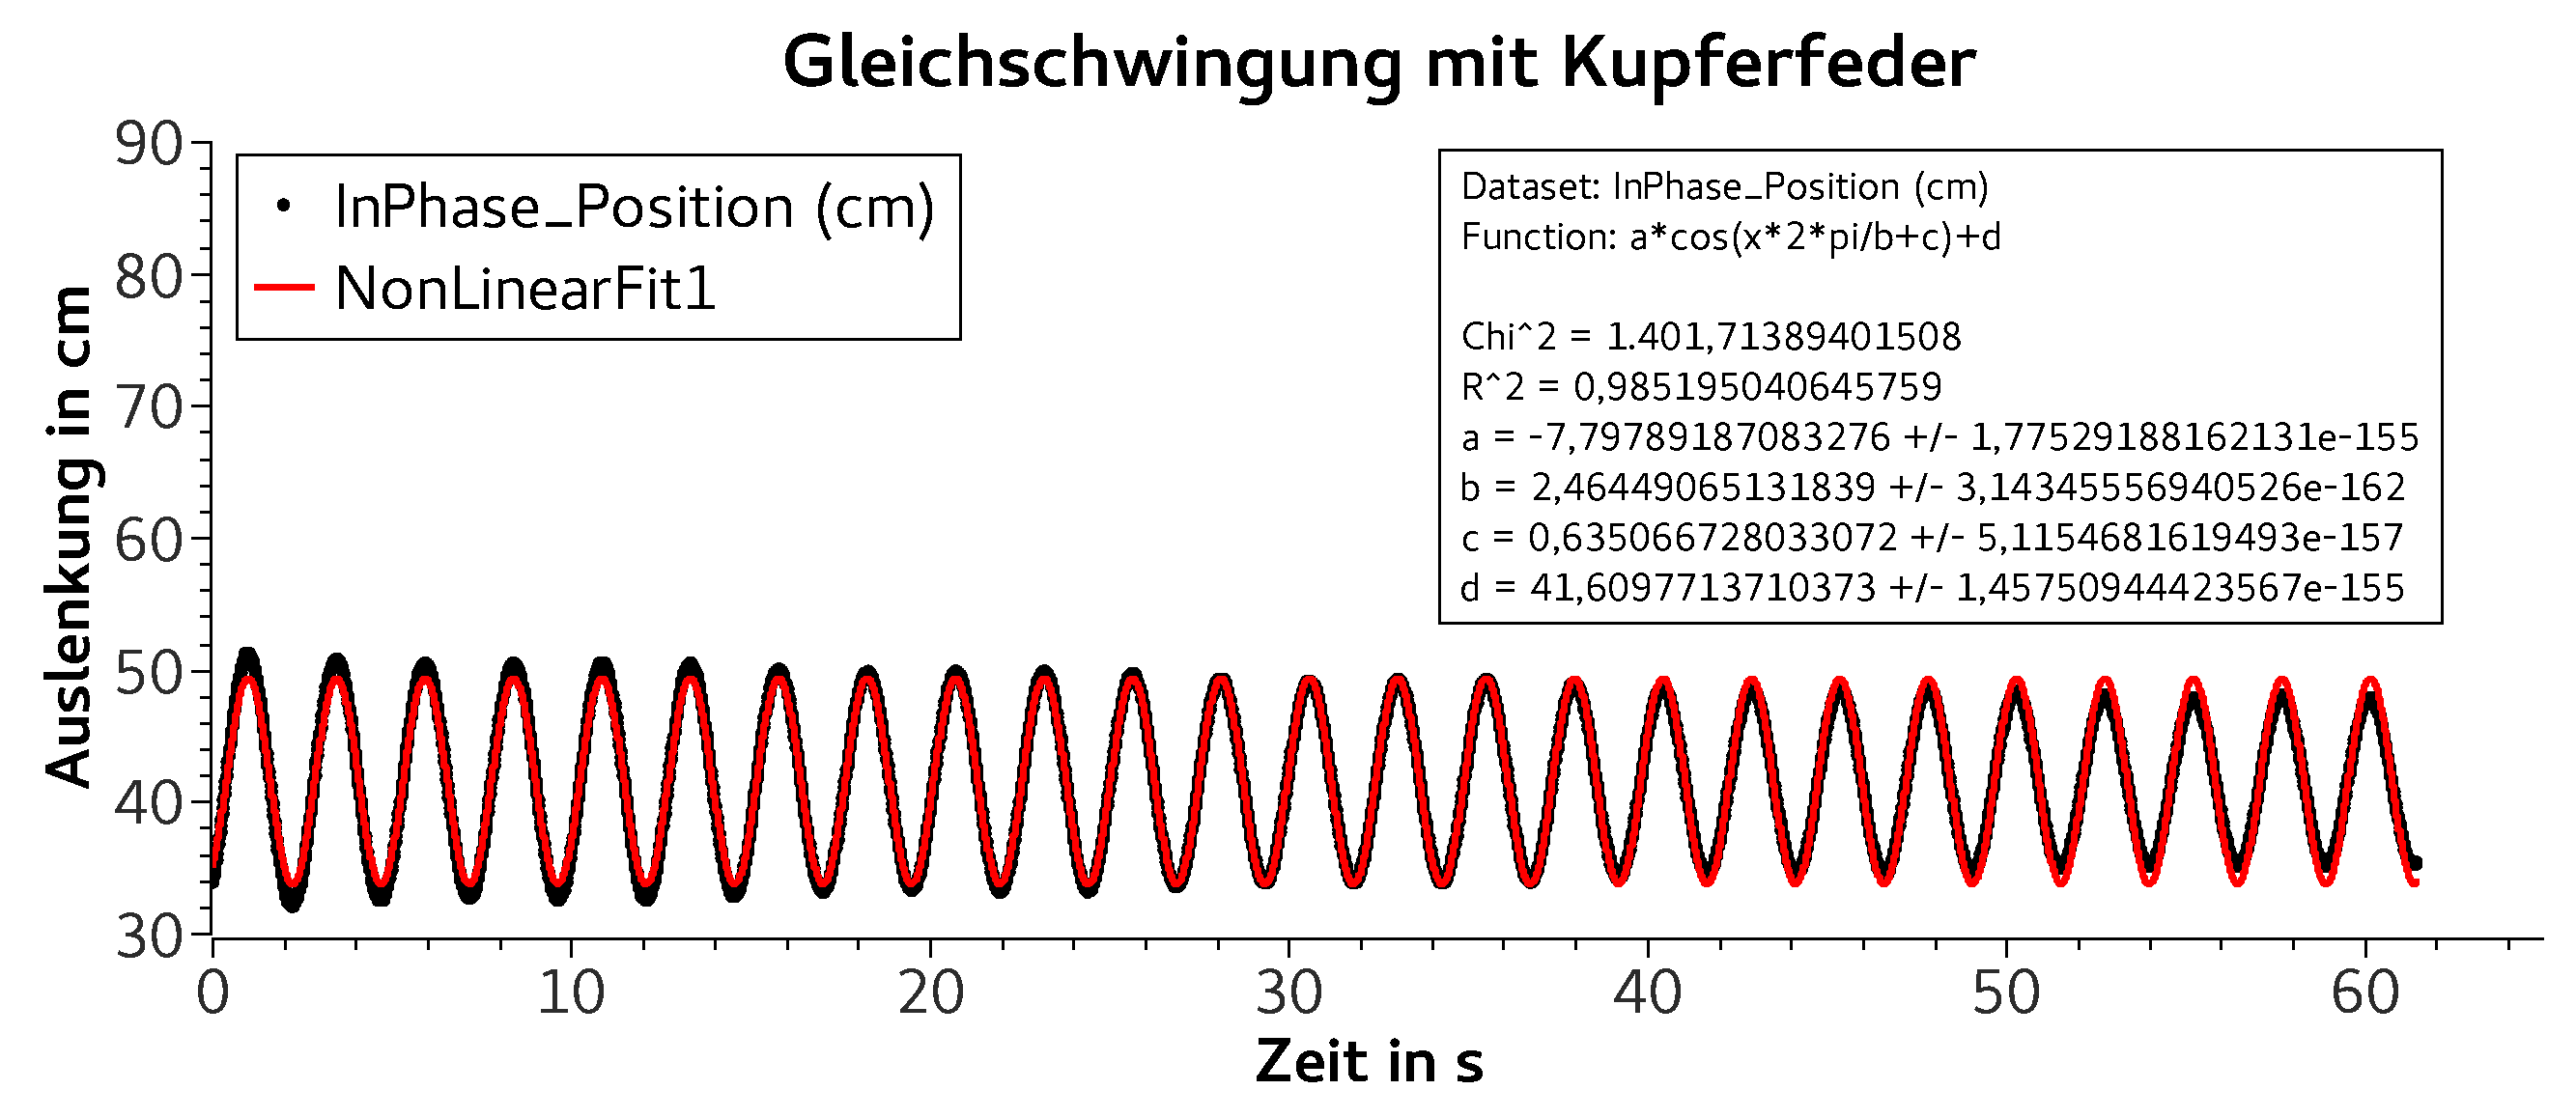
\includegraphics[width=1\textwidth]{KupferGleichschwingung}
		\centering
		\caption{Gleichschwingung mit Kupferfeder.}
		\label{KupferGleichschwingung}
		\centering
	\end{figure}

	\subsubsection*{Edelstahl}
	\begin{figure}[H]
		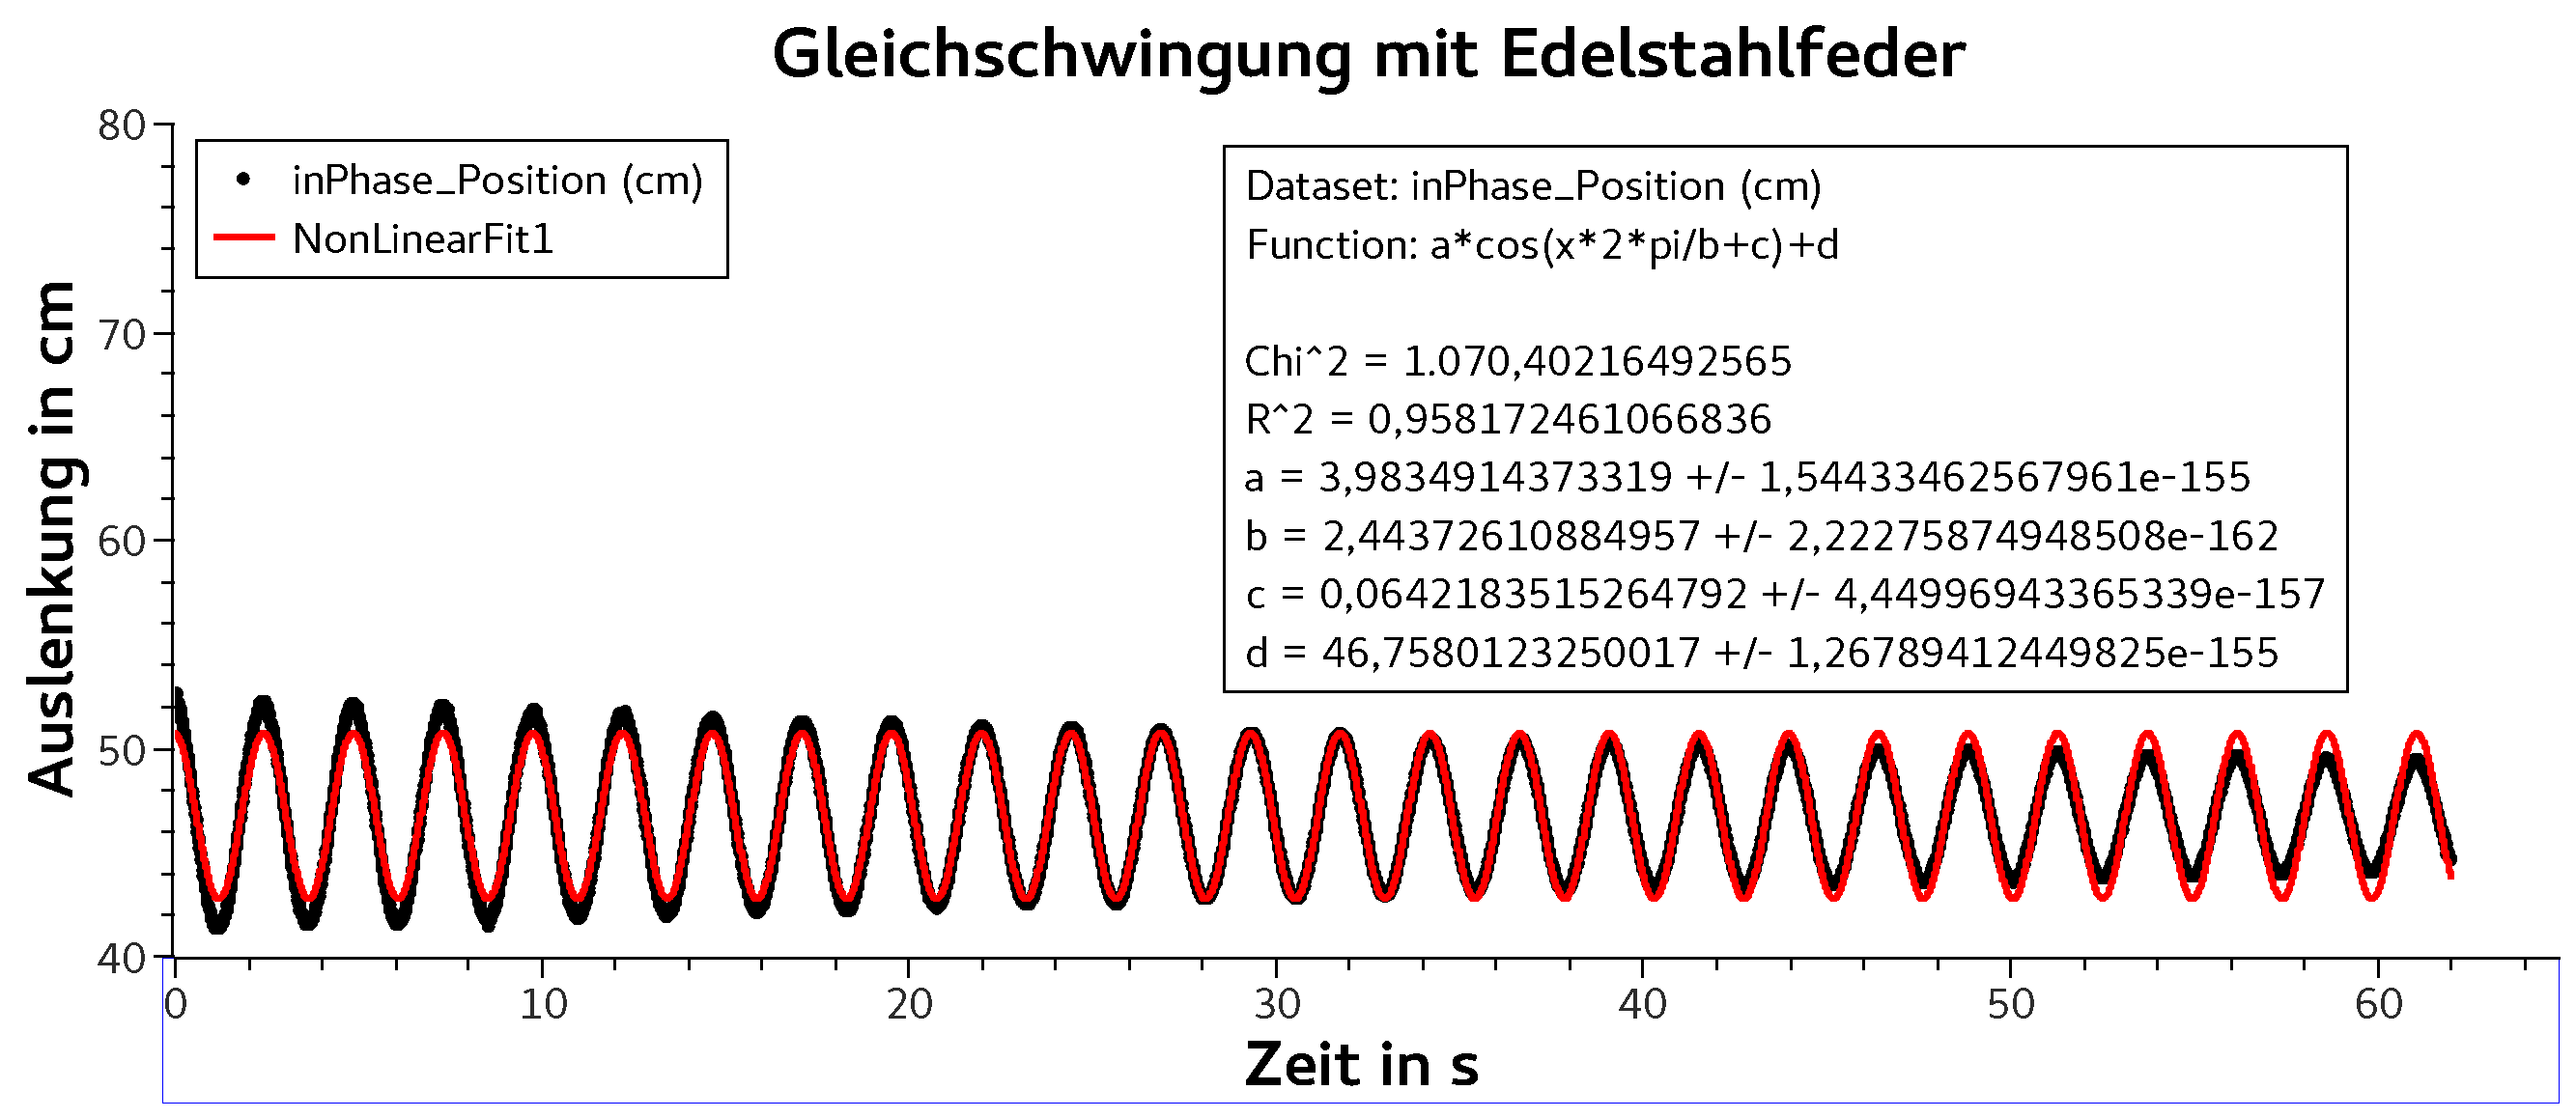
\includegraphics[width=1\textwidth]{EdelstahlGleichschwingung}
		\centering
		\caption{Gleichschwingung mit Edelstahlfeder.}
		\label{EdelstahlGleichschwingung}
		\centering
	\end{figure}


	\subsubsection{Gegenschwingung}

	\subsubsection*{Kupfer}
	\begin{figure}[H]
		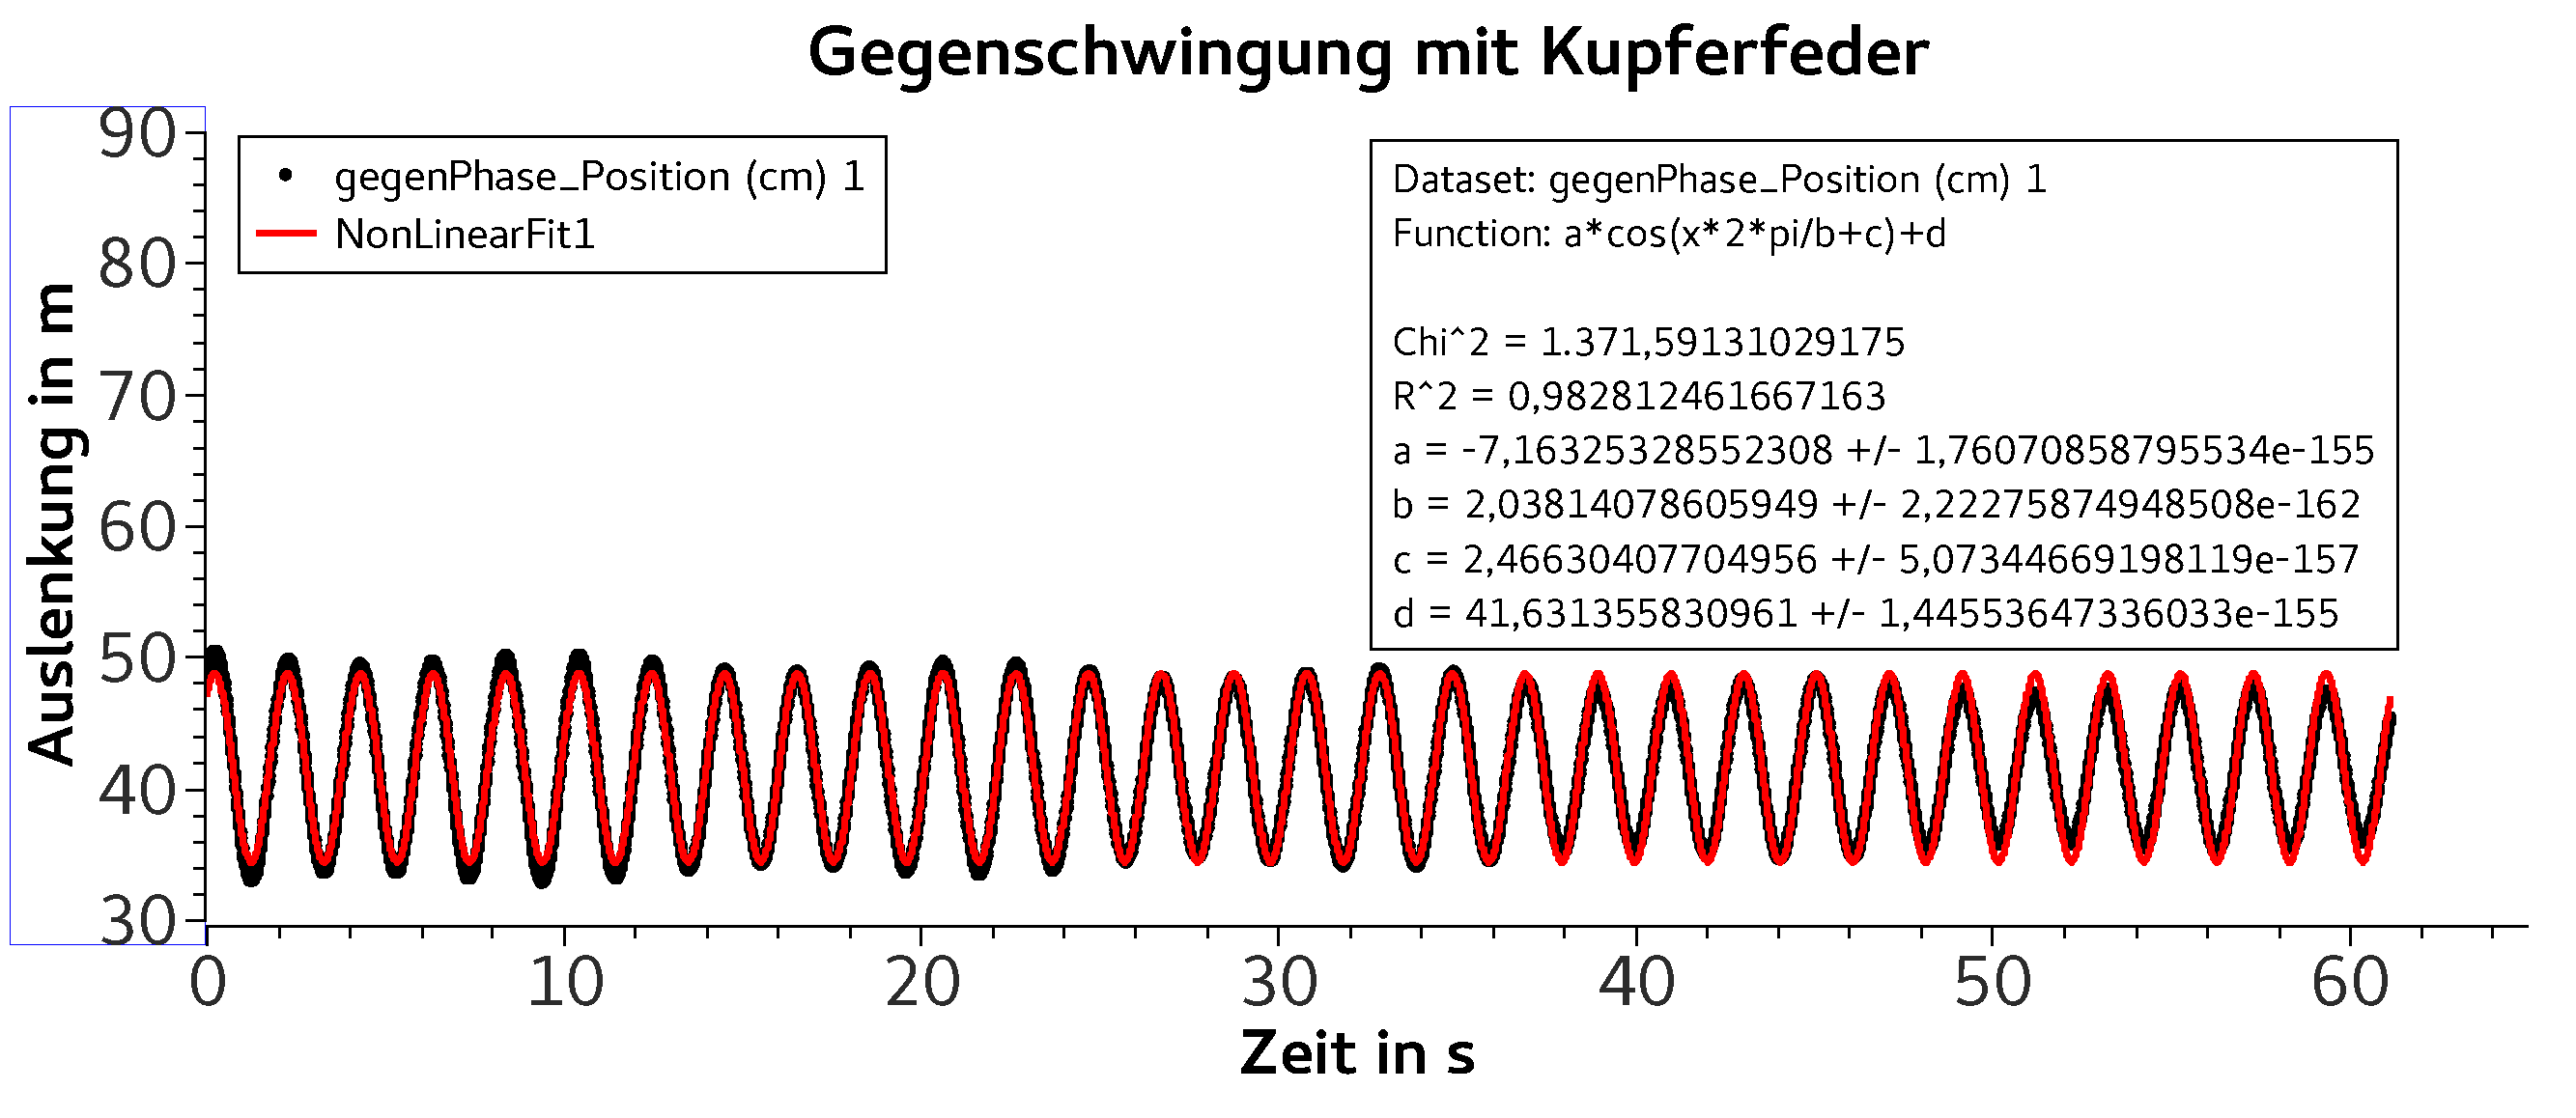
\includegraphics[width=1\textwidth]{KupferGegenschwingung}
		\centering
		\caption{Gegenschwingung mit Kupferfeder.}
		\label{KupferGegenschwingung}
		\centering
	\end{figure}

	\subsubsection*{Edelstahl}
	\begin{figure}[H]
		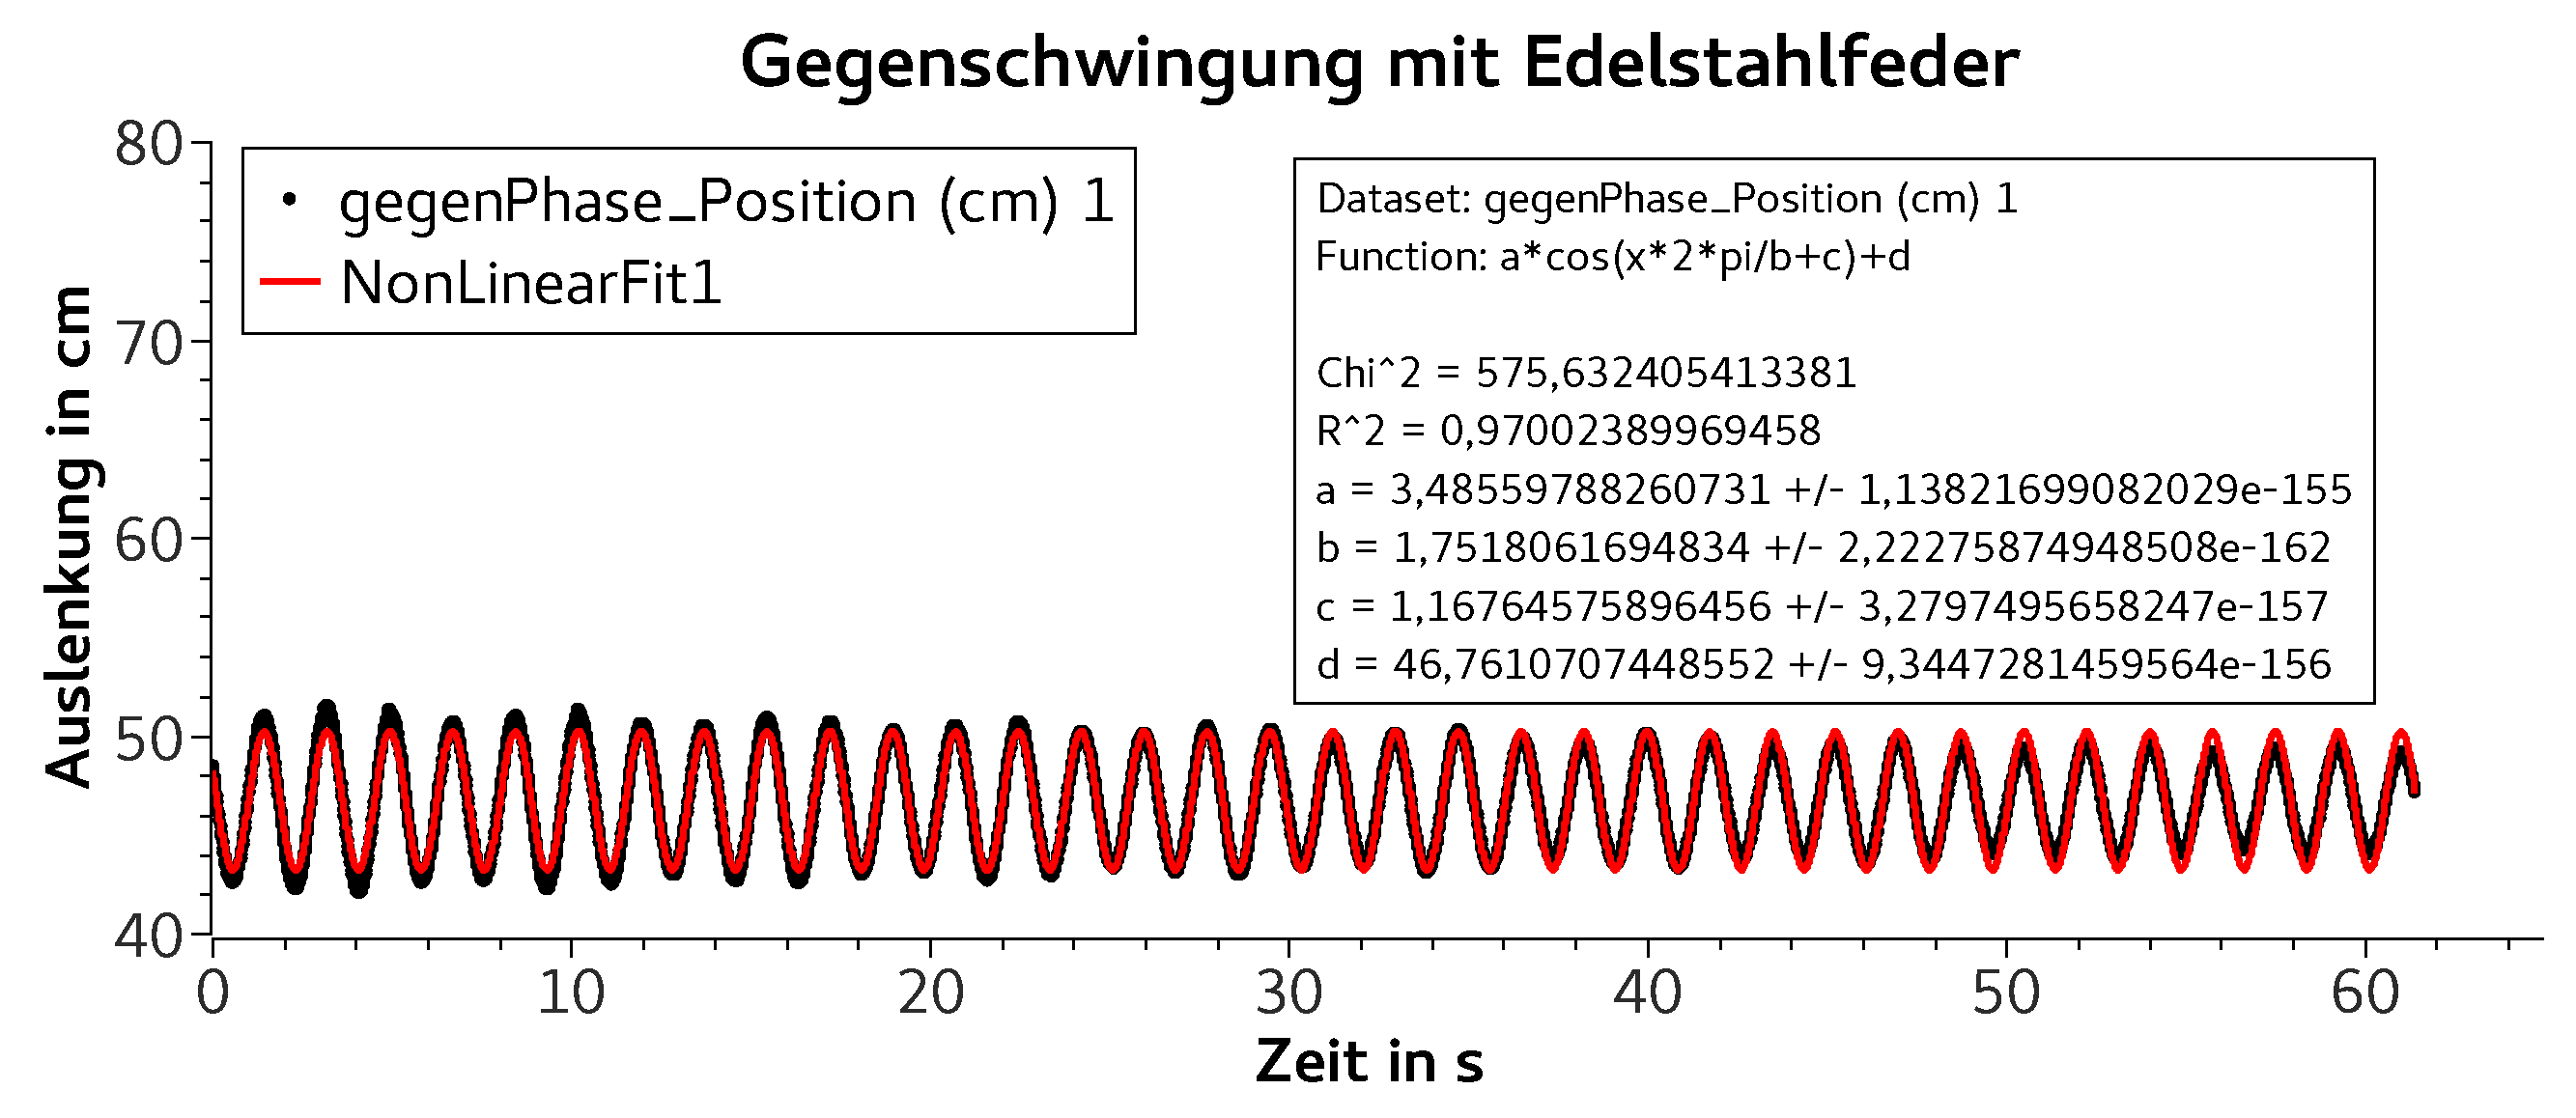
\includegraphics[width=1\textwidth]{EdelstahlGegenschwingung}
		\centering
		\caption{Gegenschwingung mit Edelstahlfeder.}
		\label{EdelstahlGegenschwingung}
		\centering
	\end{figure}



	\subsubsection{Schwebungen des gekoppelten Systems}

	\subsubsection{Vergleich der Schwingdauern}
	\subsubsection{Relative Frequenzaufspaltung}
	\subsubsection{Diskussion der Näherung}
	
	\subsubsection*{Unsicherheiten}
	Unsicherheit Ultraschallsensor pro T. \\
	Mittelwert Verrechnung. \\
	Der Ultraschallsensor misst lediglich den Abstand in der Horizontalen, das Pendel dagegen bewegt sich in einer Ebene. Da bei diesem Versuch der Fokus auf den Schwingdauern lag, ist der Fehler der somit für die Amplitude der Schwingung entsteht irrelevant.


	\subsection{Doppelpendel}
	Das Doppelpendel schwingt sehr chaotisch, d.h. es gibt auch bei nur sehr kleinen Änderungen in den Anfangsbedinungen andere Bahnen. Außerdem konnten wir zwei stabile Schwingungen beobachten, jedoch nur für ca. 5 Perioden. Danach ergaben sich minimal phasenverschobene Schwingungnen. Bei einer der stabilen Schwingungen haben beide Pendel immer in die selbe Richtung gezeigt. Die andere zeichnet sich da durch aus, dass die Pendel immer den entgegengesetzten Winkel zur Vertikalen haben. 

	\section{Schlussfolgerung}
	Näherung ist gut/schlecht. \\
	Parallelen bei Doppel- und Gekoppeltem Pendel.
	
	%\printbibliography
\end{document}
